% !TEX encoding = UTF-8
% !TEX TS-program = pdflatex
% !TEX root = ../tesi.tex

%**************************************************************
\chapter{Resoconto dello stage}
\label{cap:resoconto-stage}
%**************************************************************

%**************************************************************
\section{Pianificazione}
Prima dell'inizio del progetto di stage, insieme al mio tutor aziendale, abbiamo stilato le attività principali che avrei dovuto svolgere durante il periodo a disposizione. Queste attività sono riportate nella \hyperref[tab:pian]{tabella 2.1}.\\
Successivamente all' attività di analisi, il mio tutor, ha deciso che avrei dovuto svolgere un colloquio con lui per decidere insieme le tecnologie più promettenti e valide nel contesto di anti frode.\\
Durante i primi giorni di stage, insieme al mio tutor, abbiamo svolto vari colloqui per determinare pianificare in dettaglio le varie attività, le modalità di scelta in base al loro ambito di sviluppo e le tecnologie consigliate.

\section{Analisi}
\subsection{Introduzione}
Nei primi giorni di stage io ed il mio tutor abbiamo deciso i principali punti su cui analizzare le varie tecnologie. Questi sono conseguenti all'ambito di sviluppo dell'azienda e le tecnologie che già adotta l'azienda.\\
i punti di interesse solo:
\begin{itemize}
\item{\textbf{Licenza:}} verificare che tipo di licenza ha il prodotto, se ha una versione gratuita e che tipo limitazioni ha rispetto a quella a pagamento.
\item{\textbf{Tipo:}} verificare il tipo di tecnologia implementata, se una base di dati a grafo nativa\glsfirstoccur o non nativa\glsfirstoccur.
\item{\textbf{Modelli disponibili:}} verificare che tipi di modelli\glsfirstoccur offre.
\item{\textbf{Community:}} verificare l'ampiezza di community del prodotto in analisi, con una community molto sviluppata é possibile ricercare consigli o risoluzioni di determinati problemi nei vari \textit{forum} di riferimento.
\item{\textbf{Tecnologie sopportate nativamente(di rilievo per l'azienda):}} verificare se la tecnologia mette a disposizione un supporto a tecnologie di riferimento all'azienda quali Java o Spring.
\item{\textbf{Linguaggio di interrogazione proprietario:}} verificare se la tecnologia in analisi mette a disposizione un linguaggio di interrogazione proprietario e ottimizzato per essa, analizzando la sua espressivitá.
\item{\textbf{Supporto Tinkerpop\footnote{Tinkerpop: url= \link{http://tinkerpop.apache.org/}}:}} verificare se la tecnologia mette a disposizione il supporto ad Apache tinkerpop, sfruttando quindi un interfaccia comune, permettendo poi un passaggio ad un altra tecnologia che lo supporti a costi nulli.
\item{\textbf{Clustering\glsfirstoccur:}} verificare se la tecnologia mette a disposizione un sistema di clustering pronto all'uso, che tipo di clustering e se ha la possibilitá di eseguire query distribuite. Infine verificare se questa é disponibile nelle versione gratuita.
\item{\textbf{Security:}} verificare che sistemi di sicurezza dei dati la tecnologia mette a disposizione e se esiste la possibilità di dividere il database in zone per farle diventare accessibili solo a determinati utenti.\\

\end{itemize}
\textbf{Le informazioni necessarie all'analisi le ho riperite in primo luogo dalle documentazioni ufficiali delle case prodruttrici e successivamente dai \textit{forum} quali StackOverflow\footnote{StackOverflow: url= \link{https://stackoverflow.com/}} e Dzone\footnote{Dzone: url= \link{https://dzone.com/}}}
\subsection{Tecnologie in analisi}
Le tecnologie le ho scelte in base a quelle più diffuse o più promettenti sulla carta attraverso ricerche su internet.

\subsubsection{Sparksee(DEX)}
Sparksee\footnote{Sparksee: url= \link{http://www.sparsity-technologies.com/}} è un grafo nativo sviluppato in C++ da Spark Technologies a fine 2008 sotto nome \textbf{DEX}. Successivamente nel 2014 cambia nome in \textbf{Sparksee}.\\
Sparksee è stato il primo \textit{database} a grafo disponibile per Android e iOS.\\
Supporta tecnologie rilievo per l'azienda come Java, Maven e viene rilasciato per Linux, MacOs, Windows e per i principali sistemi operativi mobili.
La casa produttrice dichiara come \textit{use case} possibile il rilevamento di frode bancarie.\\
Questa tecnologia viene rilasciata solamente in versione con licenza commerciale ed in una accademica con il limite ad un milione di nodi.

\subsubsection{Neo4j}
Neo4j\footnote{Neo4j: url= \link{https://neo4j.com/}} è la base di dati a grafo nativa più diffusa al mondo, e, anche grazie a questo, ha una \textit{community} molto ampia. E' un \textit{software} sviluppato in Java da Neo Technology nel 2007. E' adottato da multinazionali come Microsoft, AirBnb, IBM, Ebay.\\
Neo4j ha un linguaggio di interrogazione proprietario, chimato \textbf{Chyper}, molto espressivo e ottimizzato. Supporta le tecnologie di rilievo per l'azienda, compreso Spring Data\footnote{Spring data: url= \link{http://projects.spring.io/spring-data/}}. Neo4j viene rilasciato in versione \textit{community} gratuita con nessuna limitazione di ampiezza della base di dati, senza la possibilita di eseguirlo in modo distibuito al contrario di quella \textit{Enterprise} a pagamento.

\subsubsection{ArangoDB}
ArangoDB\footnote{ArangoDB: url= \link{https://www.arangodb.com/}} è un \textit{database} multi modello sviluppato in C++ nato nel 2011. E' un \textit{database} principalmente documentale ma con collezzioni che, raccogliendo la chiave di entrata e di uscita, simulano il funzionamento a grafo. Questo permette di organizzare i documenti utilizzando il modello a grafo, documentale e chiave/valore.\\
Gli sviluppatori promettono la \textbf{flessibilità} data dalle base di dati multi modello e \textbf{velocità} paragonabile ai \textit{database} a grafo nativi.\\
ArangoDB ha un linguaggio di interrogazione proprietario simile simile ad SQL\glsfirstoccur e viene rilasciato in versione gratuita con limitazioni solo nell'ambito della sicurezza.
\subsubsection{AllegroGraph}
AllegroGraph\footnote{AllegroGraph: url= \link{https://franz.com/agraph/allegrograph/}} è un software per \textit{database} a grafo nativo sviluppato insieme agli \textit{standard} W3C\footnote{W3C: url= \link{https://www.w3.org/}} per il web semantico\glsfirstoccur  nel 2004. Supporta tecnologie di interesse all'azienda ma non ha un linguaggio di interrogazione, della base di dati, proprietario. Viene rilasciato solo con licenza commerciale a pagamento.
\subsubsection{OrientDB}
OrientDB\footnote{OrientDB: url= \link{http://orientdb.com/orientdb/}} è un \textit{software} per base di dati multi modello sviluppato in Java da uno sviluppatore italiano chiamato Luca Garulli\footnote{Luca Garulli: url= \link{https://www.linkedin.com/in/garulli}}. E' un \textit{database} principalmente documentale ma, salvando attraverso tabelle gli indici fisici di inizio e fine dell'arco, implementa anche il modello a grafo nativo. \textbf{E' il principale software capace di essere sia multi modello che a grafo nativo}.\\
Per scelta puramente commerciale hanno deciso di integrare un linguaggio di interrogazione molto simile a SQL, limitando di molto l'espressività nelle ricerche nel modello a grafo. Viene rilasciato in versione sia a pagamento che \textit{community} con nessuna limitazione di rilievo.
\subsubsection{Titan}
Titan\footnote{Titan: url= \link{http://titan.thinkaurelius.com/}} è un software in grado di sfruttare \textit{storage backend} come Apache Cassandra\footnote{Apache Cassandra: url= \link{http://cassandra.apache.org/}} per l'immagazzinamento dei dati. E' capace di astrarre i dati nello \textit{storage} ed organizzarli come se fossero a grafo, di conseguenza non utilizza una base di dati a grafo nativa.
Questa possibilità di scelta dello \textit{storage backend} lo rende molto valido se l'azienda utilizasse una tecnologia che lo supporta, questo porterebbe ad un costo di passaggio tecnologico più contenuto.\\
Titan non offre un linguaggio di interrogazione proprietario ma supporta pienamento Tinkerpop.  Viene rilasciato in licenza Apache 2\footnote{Apache 2: url= \link{https://www.apache.org/licenses/LICENSE-2.0}}.
\newpage
\subsection{Scelta tecnologica}
\begin{figure}[h!]
	\centering
	
\includegraphics[scale=0.45]{immagini/neo4j.png}
	
\includegraphics[scale=0.3]{immagini/orientdb.png}
	\caption{\textit{Logo \href{https://neo4j.com/}{Neo4j} e \href{http://orientdb.com/orientdb/}{OrientDB}}}
\end{figure}
Dopo un colloquio dove ho mostrato al mio tutor i risultati dell'analisi, in comune accordo abbiamo scelto le due tecnologie più promettenti ed interessanti.\\
Abbiamo stato scelto \textbf{Neo4j} per il suo linguaggio di interrogazione molto espressivo, la sua diffusione a livello mondiale che porta ad una community molto attiva.\\
Infine abbiamo scelto anche \textbf{OrientDB} essendo il \textit{database} multi modello più promettente sulla carta che organizza i dati come uno a grafo nativo.

\section{Sviluppo del prototipo}
\subsection{Base di dati}
In base al problema descritto nella \hyperref[sec:prob]{sezione 2.1.1} e dinamiche di Smash\textregistered ho organizzato i dati, per tutti e due i \textit{database}, nel seguente modo:
\begin{itemize}
\item{\textbf{Nodi:}}
\begin{itemize}
\item{\textbf{EntityId:}} è il nodo che rappresenta un utente di una banca, esso può sia svolgere \textbf{transazioni} verso un \textit{AccountId} che avere \textbf{relazioni di appartenenza} verso un, o più, \textit{AccountId}.
\item{\textbf{AccountId:}} è il nodo che rappresenta una coordinata bancaria ad esempio un iban, esso può avere transazioni verso altri \textit{AccountId} ed avere massimo una relazione di appartenenza da un \textit{EntityId} a questo nodo.
\end{itemize}
\item{\textbf{Archi:}}
\begin{itemize}
\item{\textbf{TRANSACTION:}} è l'arco che rappresenta una transazione, questo può provenire da un \textit{AccountId} o \textit{EntityId} verso un \textit{AccountId}. Questo ha diverse proprietà tra cui di obbligatorie la data di avvenuta transazione, l'importo e la valuta, e di non obbligatorie come la città e il paese dove è stata eseguita la transazione.
\item{\textbf{OWN:}} è l'arco che descrive la relazione di appartenenza da un \textit{EntityId} ad un \textit{AccountId}.Un \textit{EntityId} può avere un numero a piacere di relazioni di appartenenza, al contrario un \textit{AccountId} può avere al massimo un arco entrante di tipo \textit{OWN}.
\end{itemize}
\end{itemize}
\newpage
\begin{figure}[!ht]
	\centering
	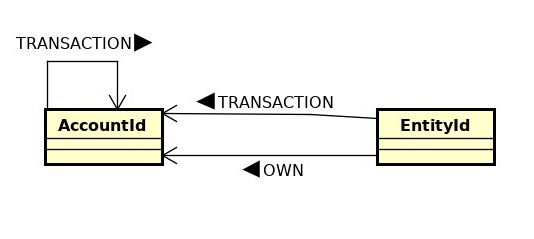
\includegraphics[scale=0.4]{immagini/graph.jpg}
	\caption{\textit{Schema della base di dati}}
\end{figure}
\textbf{A causa i problemi legati alle politeche della protezione dei dati sensibili, non ho potuto utilizzare dati reali per il popolamento dei \textit{database} ma ho dovuto creare un progetto per la creazione di dati casuali.}

\subsection{Prototipo}
Ho deciso di dividere il prototipo in più progetti sotto l'unico aggregato Maven\glsfirstoccur chiamato \textit{xtn\textunderscore research\textunderscore graphdbs}. Questa tecnica l'ho utilizzata per gestire tutte le versioni delle dipendente in un unico file di configurazione, e, sopratutto, per avere la comodità di eseguire la \textit{build} di tutti i progetti in un unico comando, lasciando a Maven l'onere di risolvere tutte le dipendenze.\\
Il diagramma dei \textit{package} e le relative dipendenze è il seguente.
\begin{figure}[h!]
	\centering
	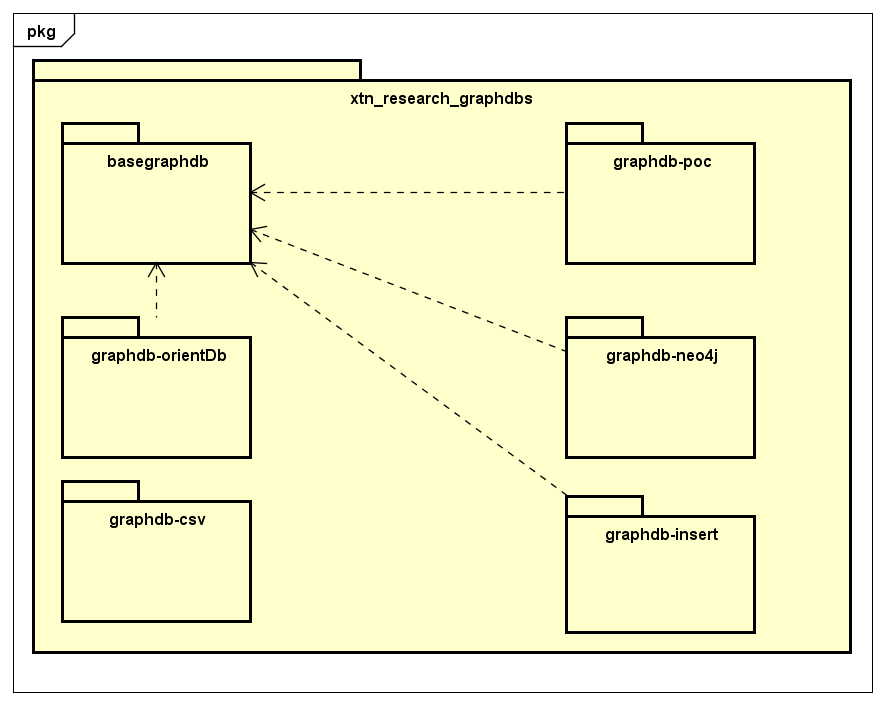
\includegraphics[scale=0.55]{immagini/packages.png}
	\caption{\textit{Diagramma dei package del prototipo}}
\end{figure}

\subsubsection{basegraphdb}
\textit{Basegraphdb} é il progetto che contiene le varie interfacce comuni tra cui \textit{ReputationController}. Questa é l'interfaccia comune per gestire la reputazione delle varie entitá presenti nei vari \textit{database}. Ogni implementazione, quindi sia \textit{graphdb-neo4j} che \textit{graphdb-orientDb}, conterrà una classe che la implementerà.
\subsubsection{graphdb-orientdb}
\textit{Graphdb-orientDb} é il progetto per la gestione della reputazione tramite OrientDB, esso ha all'interno una classe chiamata \textit{ReputationControllerOrientDb} che implementa \textit{ReputationController}. Questa implementazione usa Tinkerpop\footnote{Tinkerpop: url=\link{http://tinkerpop.apache.org/}} per interfacciarsi con il \textit{database}.
\subsubsection{graphdb-neo4j}
\textit{Graphdb-neo4j}́ è il progetto per la gestione della reputazione tramite Neo4j, esso ha all'interno una classe chiamata \textit{ReputationControllerNeo4j} che implementa \textit{ReputationController}. Questa implementazione utilizza \textit{Spring Data Neo4j} per interfacciarsi 



\section{Verifica e validazione}
Descrizione e resoconto dell'attività di verifica e validazione.

\section{Conclusioni}

Descrizione delle conclusioni che sono emerse grazie all'analisi e da PoC

